\section{Subsequence Match Merging}\label{sec:smm}
In this section, we introduce our second defense mechanism (\contribution{3.2}) called \textit{subsequence match merging} (SMM)~\cite{Saglam2024d}.
While there is some research to counteract such automated obfuscation attacks, these approaches face two crucial challenges~\cite{Saglam2024b}.
First, \textit{language-dependence}: Defense mechanisms are often highly language-specific, hindering straightforward generalization or transferability across different programming languages.
Second, \textit{attack-type-dependence}: Defense mechanisms are usually only tailored to one specific attack vector, thus lacking broad resilience. While highly efficient against the intended attacks, they provide little resilience for other attack types.
Thus, they serve little protection against unknown attacks. Such emerging attacks, however, constitute the most challenging scenarios.
However, with the recent rise of large language models and their \textit{commoditization} via tools like ChatGPT~\cite{ChatGPT}, addressing emerging attacks is more crucial than ever~\cite{ChatGPTGuide}. 

Given these challenges, we introduce a novel approach called subsequence match merging to bolster the obfuscation resilience of today's state-of-the-art software plagiarism detectors.
%
All obfuscation attacks, whether known or unknown, have to disrupt the matching of code fragments to be effective~\cite{DevoreMcDonald2020}. Thus, they must affect the detectors' internal program representation~\cite{Saglam2024b}.
%
To this end, obfuscation attacks try to alter the structural properties of a plagiarized program.
%
Our approach iteratively merges neighboring fragment matches in pairs of linearized programs according to a well-designed heuristic until no more neighboring pairs remain. This process effectively reverses the effects of obfuscation, enhancing the detection of obfuscated plagiarism while minimizing false positives.
%
As our approach operates solely on the internal linearized representations of programs, it is entirely language-independent and not limited to a single obfuscation attack type.
Thus, subsequence is not limited in its effectiveness to semantic-preserving or semantic-agnostic obfuscation attacks.
It is also capable of defending against semantic-deviating obfuscation attacks.
We thus provide a robust and versatile approach for a broad spectrum of known and unknown obfuscation attacks.

\begin{factsheet}{Overview: Subsequence Match Merging} 
    \begin{description}[style=multiline,leftmargin=5.5cm]
        \item[Core Principle] Revert Match Splitting Heuristically
        \item[Targeted Obfuscation Attack] Unspecified, Broad Resilience
        \item[Language Family] Programming and Modelling Languages
        \item[Language Dependence] Language-Independent
        \item[Performance Impact] Moderate
        \item[Main Scalability Determinant] Number of Matches
        \item[Integration Complexity] Low
    \end{description}
\end{factsheet}

\subsection{Targeted Obfuscation Attacks}

Subsequence match merging is an algorithm that heuristically searches among all matched subsequence pairs between two linearized programs to find \textit{neighboring} matches that can be merged into a single one, subsuming the (unmatched) gap between them. This is done iteratively until no more neighboring pairs are found. This approach effectively reverts the effects of obfuscation attacks on the linearized program.
As discussed in \autoref{cha:threatmodel}, all obfuscation attacks must affect the token sequence, thus interrupting the matching, to be effective. 

Subsequence match merging relies solely on matching subsequences in the internal token-based representation, independent of the underlying programs. This makes it inherently language-independent. Furthermore, our approach relies only on the structural properties of all matched subsequences but does not consider the semantics of the corresponding tokens, thus making it attack-type-independent.
Therefore, our approach provides resilience against any potential obfuscation attack.
Consequentially, this subsequence match merging does not target a specific attack type. Instead, it aims to provide broad resilience that can be layer with other defense mechanisms.
In detail, it offers significant resilience against weaker obfuscation attacks and some resilience against stronger obfuscation attacks.

As discussed, all token-based plagiarism detectors employ a cut-off threshold, below which matched code fragments are ignored to avoid false positives. This threshold, often called minimum match length (MML)~\cite{Saglam2022}, defines the minimal number of tokens required for two matching subsequences to be counted toward the similarity score.
Thus, the minimum match length controls the sensitivity of the comparison algorithm: if set too low, it increases the similarity but also the likelihood of false positives and vice versa.
Obfuscation attacks affect the detection by splitting up matching subsequences of tokens until enough subsequences are small enough to fall below the minimum match length and are thus ignored.

Thus, our approach aims to reverse this by merging neighboring blocks of matches. The merging operates heuristically by assessing how close \textit{neighboring} matches are, regardless of whether the alterations initially involved insertion, deletion, or reordering. By carefully selecting the matches to merge, we ensure a negligible impact on the false positive rate.

\subsection{Neighboring Matches}
A key concept in our approach is \textit{neighborhood} of matches.
We define matches as neighbors if they directly follow each other in the same order in both token sequences of a program pair. \textit{Directly} refers to having no other matches in between on either side of the pair. This, however, does explicitly not include unmatched tokens.

\begin{theorem}[Neighboring Matches]\label{def:neighbors}
Let \( (t_i) \) and \( (t'_i) \) be the token sequences of two programs, and let \( (m_i) \) and \( (m'_i) \) be subsequences of matching tokens in \( (t_i) \) and \( (t'_i) \), respectively. Two matches \( (m_i) \) and \( (m'_i) \) are considered neighbors if:
\begin{align*}
(m_i) \sqsubseteq (t_i), \quad (m'_i) \sqsubseteq (t_i), \quad (m_i) \sqsubseteq (t'_i), \quad (m'_i) \sqsubseteq (t'_i),
\end{align*}
and
\begin{align*}
(m_i) \prec_{(t_i)} (m'_i), \quad (m_i) \prec_{(t'_i)} (m'_i),
\end{align*}
where \( \prec \) denotes the canonical order of subsequences in a token sequence. Specifically, it indicates the natural order based on the indices of the tokens within their respective sequences.
\end{theorem}

\begin{figure}[b]
    \centering
    
\includegraphics[width=\linewidth]{figures/algorithm/neighbors.pdf}
    \caption[Neighboring Subsequence Matches]{Two tokenized programs with four subsequence matches $(a_i)$--$(d_i)$, of which only the matches $(c_i)$ and $(d_i)$ are neighbors.}
    \label{fig:neighbors}
\end{figure}

To illustrate \autoref{def:neighbors}, \autoref{fig:neighbors} depicts four matches between the token sequences of two programs. The matched subsequences are in the order $((a_i), (b_i), (c_i), (d_i))$ in the original program and $((b_i), (a_i), (c_i), (d_i))$ in the variant. Therefore, matches $(a_i)$ and $(b_i)$ would not be considered neighbors, as their subsequence order is inconsistent across both programs. Matches $(a_i)$ and $(c_i)$ are not neighbors, as the corresponding subsequences in the original are interrupted by match $(b_i)$, which also is the case for $(b_i)$ and $(c_i)$ in the variant. In contrast, match $(c_i)$ and match $(d_i)$ are considered neighbors because they follow each other in the same order and are only separated by non-matching tokens.

Neighboring subsequence matches represent matching code fragments in the original programs. For instance, in \autoref{tab:running-example}, lines 1--3 and 6--8 match in the original program and in the variant. These lines appear in the same order and have no other matching segments in between, thus leading to a pair of neighboring matches in the token sequences. The non-identical statements that separate these neighboring matches are the inserted line 4 and the altered line 5.
%Neighboring token matches thus represent matching code fragments separated by non-identical statements.

\subsection{Algorithm}
\label{subsec:smm-algorithm}
Subsequence match merging operates as outlined in \autoref{alg:matchMerging}. The algorithm takes the token sequences of two programs and their matching subsequences as input. Note that this includes all matches, including those who fall below the minimal match length of the plagiarism detector. Initially, we compute which matching subsequences qualify as neighboring matches. If a pair of neighboring matches meets the merging criteria, we merge them and eliminate the gap in both token sequences.
This involves effectively ignoring the unmatched tokens between the neighboring matches. After each merge, we recompute the neighbors and repeat this process until no more neighboring matches that fulfill the merging criteria are found. This means that merged matches can be merged with others in the following iterations.
%
Our merging criteria are defined as follows:
\begin{description}[style=unboxed,leftmargin=0cm]
 \item[Minimal Neighbor Length:] Both neighboring matches must exceed a specific length in tokens (for example, matches with a length above two tokens).
 \item[Maximal Gap Size:] The mean gap of unmatched tokens between these neighboring matches must not exceed a specific size (for example, a gap below six tokens). 
\end{description}

More formally, we thus merge all neighboring merges where both thresholds mentioned above are fulfilled.
This is defined as follows.

\begin{theorem}[Neighbor Length Fulfillment]\label{def:neighbor-length}
Two neighboring matches \((a_i)_{i=1}^l\), \((b_j)_{j=1}^n\) according to \autoref{def:neighbors} and \autoref{def:matching-tokens} fulfill the minimal neighbor length threshold \(\ell_{\text{MNL}}\) iff
\[
    \ell_{\text{MNL}} \leq |a_i| = l \quad \land \quad \ell_{\text{MNL}} \leq |b_j| = n \,.
\]
\end{theorem}

\begin{theorem}[Gap Size Fulfillment]\label{def:gap-size}
Two neighboring matches \((a_i)_{i=1}^l\), \((b_j)_{j=1}^n\) according to \autoref{def:neighbors} and \autoref{def:matching-tokens}, which are separated in the token sequences of two programs by the subsequences \((c_k)_{k=1}^p\), \((d_m)_{m=1}^q\), fulfill the maximum gap size threshold \(\ell_{\text{MGS}}\) iff
\[
    \ell_{\text{MGS}} \geq \frac{|c_k| + |d_m|}{2} = \frac{p + q}{2} \,.
\]
\end{theorem}


\begin{algorithm}
\caption{Subsequence Match Merging}\label{alg:matchMerging}
\begin{algorithmic}[1]
  \Require{$tokenSequences, originalMatches$}
  \State $matches \gets originalMatches$
  \State $neighbors \gets \textproc{computeNeighbors}(matches)$
  \State $numberOfMerges \gets 0$
  \Repeat
    \For{each $neighborPair \in neighbors$}
      %\If{$\text{average size of } gapTokens \leq gapSizeThreshold$}
      \If{$\textproc{satisfiesMergingCriteria}(neighborPair)$}
        \State $mergedMatch \gets \textproc{mergeNeighbor}(neighborPair)$
        \State $matches \gets matches \cup \text{mergedMatch}$
        \State $matches \gets matches \setminus \text{neighborPair}$
        \State $numberOfMerges \gets numberOfMerges +1$
      \EndIf
    \EndFor
    \State $neighbors \gets \textproc{computeNeighbors}(matches)$
  \Until{no more valid merges}
  \If{$numberOfMerges \geq minimumMerges$}
    \State \Return $\textproc{pruneMatches}(matches)$
  \Else
    \State \Return $originalMatches$
  \EndIf
\end{algorithmic}
\end{algorithm}

Our algorithm merges pairs of neighboring matches when both have sufficient lengths and are separated by minimal tokens, indicating the pair represents a formerly single uninterrupted match. Our heuristic is based on thresholds for minimum neighbor length and maximum gap size, merging matches that meet these criteria.
Note that the neighbor length fulfills a purpose similar to the minimal match length. It controls the sensitivity of the approach.
%
After merging, we need to filter any remaining matches that fall below the minimum match length to ensure that the resulting matches do not violate the assumptions of the plagiarism detector. This means some merged matches must not be included, as they may fall below the minimum match length threshold (\textproc{pruneMatches} in \autoref{alg:matchMerging}).
By considering matches below the minimum match length threshold before the pruning step, our approach can merge matches that the plagiarism detector would not have considered. Essentially, this allows the fragmentation of matches to be reversed, thus reverting the effects of obfuscation attacks.
Finally, we check how many neighboring matches were merged. When this number is below a threshold called \textit{minimal merges} (MM), the merged matches are dropped, and the original ones are used. This threshold is a safeguard to reduce the impact on pairs or unrelated programs.

\autoref{fig:fullMatchMerging} illustrates the subsequence match merging algorithm as defined in \autoref{alg:matchMerging} for our running example in \autoref{tab:running-example}. It shows how the token sequences of two programs are aligned via subsequence match merging in two steps. 
\textit{Step 0} displays the token sequences of the original program and its obfuscated variant from \autoref{tab:re-tokens}, along with the matching subsequences between them. For illustrative purposes, let the minimum match length threshold be four tokens, resulting in a similarity score of 0\% because all three matches fall below this threshold.
Due to obfuscation, the matching subsequences are interrupted, and all matches fall below the minimum match length and are thus omitted.
In step 1, we merge the first two subsequence matches, which are only separated by a single token in the variant sequence. Both matches are at least two tokens long and only separated by \(\frac{0 + 1}{2} = 0.5\) tokens.
After merging, the match length increases to 5, thus raising the similarity score to 58.8\%.
In \textit{Step 2}, we assess the remaining pair of neighbors which also meet the threshold criteria.
We merge the remaining two subsequence matches, which are now separated by a single token in the original sequence. Again, both matches are long enough and are only separated by \(\frac{1 + 0}{2} = 0.5\) tokens. Since we cannot find any more matches to merge, we terminate. As we eliminate the separating tokens during the merging, the resulting match is above the minimal match length, and the token sequences of both programs are now considered identical.
Merging them raises the similarity score to 100\%, thus reverting the obfuscation demonstrated in the running example.

\begin{figure}
\centering
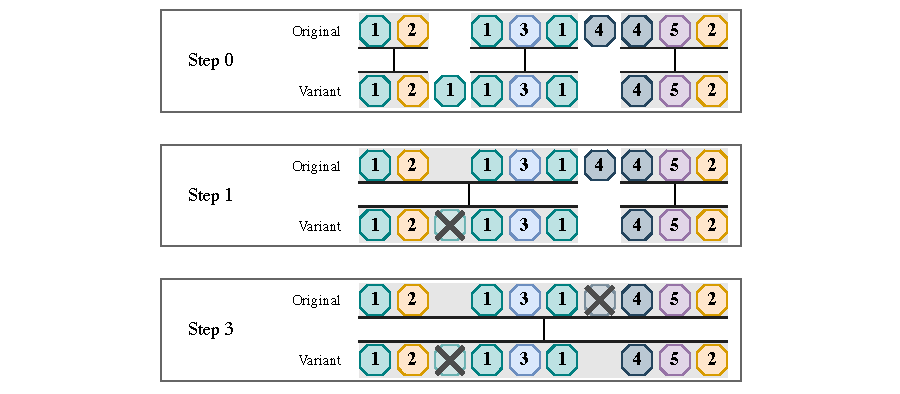
\includegraphics[width=\linewidth]{figures/algorithm/steps.pdf}
\caption[Subsequence Match Merging Example]{Steps of the subsequence match merging for the running example in \autoref{tab:re-tokens} (minimum match length = 4, minimum neighbor length =, 2 and maximum gap-size = 1).}
\label{fig:fullMatchMerging}
\end{figure}

\subsection{Complexity}
The runtime complexity of the \textit{Subsequence Match Merging} algorithm depends on the number of matches $m$ and the efficiency of merging operations.
The runtime complexity depends on the three main operations: Neighbor computation, merging, and pruning.
The neighbor computation scans all matches sequentially to identify adjacent pairs with a $O(m)$ complexity.
Merging a pair of neighbors is an $O(1)$ operation, while pruning matches after all iterations also requires $O(m)$ time.
We check each neighboring pair for the merging criteria and repeat this until no more merges occur.

In the worst case, each algorithm iteration performs an $O(m)$ neighbor computation and processes up to $O(m)$ merges, with a maximum of $m$ iterations if only one merge occurs per iteration. This results in a worst-case complexity of $O(m^2)$. Conversely, in the best case, where merges significantly reduce the number of matches (e.g., halving the matches in each iteration), the algorithm performs $O(\log m)$ iterations, with each iteration requiring $O(m)$ operations for neighbor computation and merging. Consequently, the best-case complexity is $O(m \log m)$.

The length of the token sequences limits the number of matches. For the sake of the complexity, $m$ can thus also be seen as the length of the longer sequence. As the worst-case runtime complexity for greedy string tiling per program pair is \( O(m^3) \) (see \autoref{sec:found-jplag}), subsequence match merging does not increase the runtime complexity of the plagiarism detection process.

\subsection{Hyperparameters}
To fine-tune the algorithm, we provide two primary hyperparameters: the minimum neighbor length and the maximum gap size (see \autoref{subsec:smm-algorithm}). These can be adjusted to, for example, fit the algorithm to a specific dataset.
Both thresholds are critical for tuning the heuristic's aggressiveness in deciding which neighboring matches to merge. Setting a low neighbor length and a high gap size threshold tends to merge unrelated matches, increasing false positives. Conversely, a high neighbor length and a low gap size limit the effectiveness of our approach by failing to detect most instances of plagiarism. 

We conducted a grid search for a suitable default parameterization to address the trade-off between precision and recall.
We explored neighbor length values from 1 to the minimum match length. The minimum match length was chosen as the upper threshold, as matches above this threshold have already been detected. Furthermore, we explore gap size values from 1 to 20. We chose 20 as the upper threshold, representing a significant code fragment. During our grid search, this was confirmed, as the best results occur far below the threshold of 20. After evaluating each combination across various real-world datasets consisting of different assignment types, sizes, and different programming languages, as well as with varying obfuscation attacks, we observed that a minimum neighbor length of 2 and a maximum gap size of 6 yields the strongest resilience against obfuscation attacks.
To recap, this means that neighboring matches are merged only if each match spans at least two tokens and six or fewer tokens separate them.
Thus, we propose these values as default parametrization. However, we also recommend adjusting these hyperparameters for the dataset at hand when using our approach.

Finally, for the number of minimal merges, we recommend a low value of between three and five. By choosing a conservatively low value here, we ensure that this safeguard does not affect the performance of the algorithm for obfuscated programs.

\subsection{Observed Impact}\label{sec:smm-impact}
This section presents initial observations on the effectiveness of subsequence match merging based on real-world data. It is important to note that this is not intended as a comprehensive evaluation but aims to provide an empirical perspective on how the defense mechanism performs in practical scenarios.

When applying subsequence match merging to an exemplary dataset from programming assignments and analyzing its impact, we observe a distinct difference between unrelated program pairs and those where one program was plagiarized and obfuscated to create the other. For instance, in cases of obfuscation through statement insertion using PlagGen~\cite{Broedel2023}, unrelated program pairs experience an average of 3.64 individual merges. In contrast, plagiarism pairs undergo an average of 73.90 merges. This indicates that the merging criteria of the algorithm rarely fulfilled for unrelated solutions but frequently fulfilled for plagiarism pairs, demonstrating the effectiveness of our heuristic. For this exact purpose, we designed the safeguard via a minimal number of merges. 

%\todo{Empiric results PP-19:}
%\todo{27 Plags: MaxGap{count=1552, sum=4945, min=1, average=3,186211, max=12}}
%\todo{351 Unrelated: MaxGap{count=1276, sum=3272, min=1, average=2,564263, max=12}}
%\todo{Means 73.90 individual merges per plag pair but only 3.64 for unrelated pair}

When varying the hyperparameters of the SMM algorithm for the aforementioned dataset, we can observe how the parameterization affects the effectiveness of the algorithm.
\autoref{fig:mm-nl} illustrates this for a varying minimal neighbor length. As previously discussed, this controls how long neighboring matches must be to qualify them for merging. The original and plagiarized programs achieve almost identical similarity values without match merging. The lower the minimal neighbor length, the clearer the separation becomes. We can see how this parameter controls the aggressiveness of the merging. Lower values lead to fewer individual merges and vice versa.

Next, \autoref{fig:mm-nl} illustrates the impact of the hyperparameters for a varying maximal gap size. The gap size controls how many tokens can separate two neighboring matches to still qualify them for merging. Again, without merging, the similarity values collapse. For the gap size, the effectiveness increases when increasing the parameter. However, the effects are less strongly pronounced compared to the neighbor length. Furthermore, the impact of an increasing gap size stagnates at a particular value. In the case of \autoref{fig:mm-nl}, this happens at a gap size of 5 tokens.

In Summary, we can observe that subsequence match merging increases the similarity of plagiarism pairs while maintaining a minor impact on the original and unrelated pairs. With this, subsequence match merging improves the resilience against obfuscation attacks.


\begin{figure}[p]
\centering
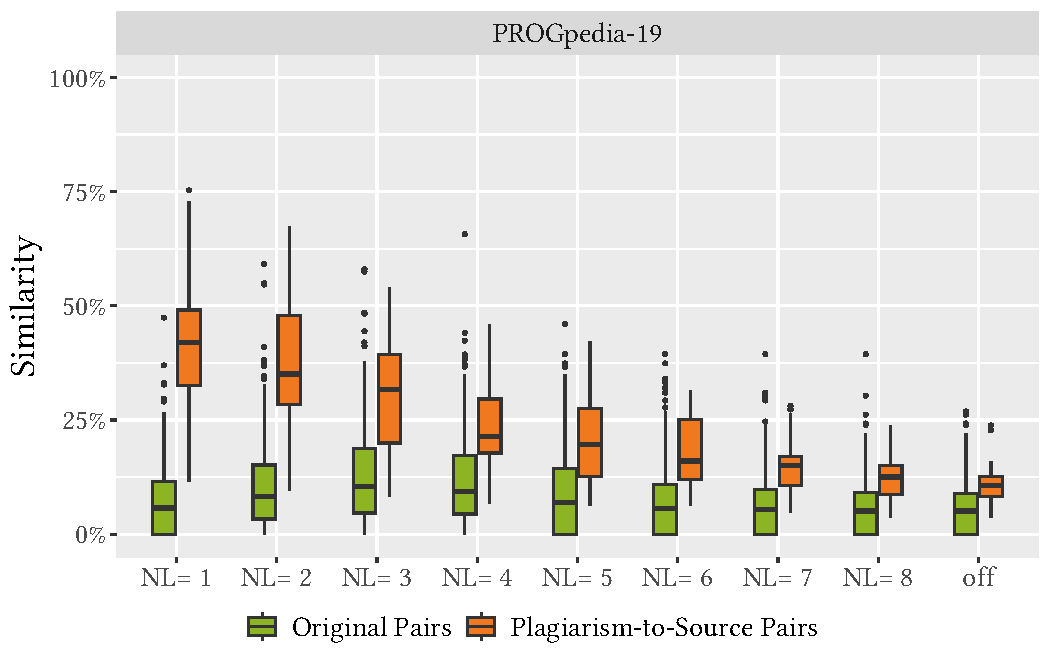
\includegraphics[width=0.95\linewidth]{figures/algorithm/eval-mm-NL_avg.similarity.pdf}
\caption[Impact of the Neighbor Length]{Impact of the hyperparameter neighbor length (NL) for a programming assignment dataset~\cite{paiva2023} and plagiarized programs via insertion-based obfuscation via PlagGen~\cite{Broedel2023}. Plagiarism pairs should be high, while original pairs should be low.}
\label{fig:mm-nl}
\end{figure}

\begin{figure}[p]
\centering
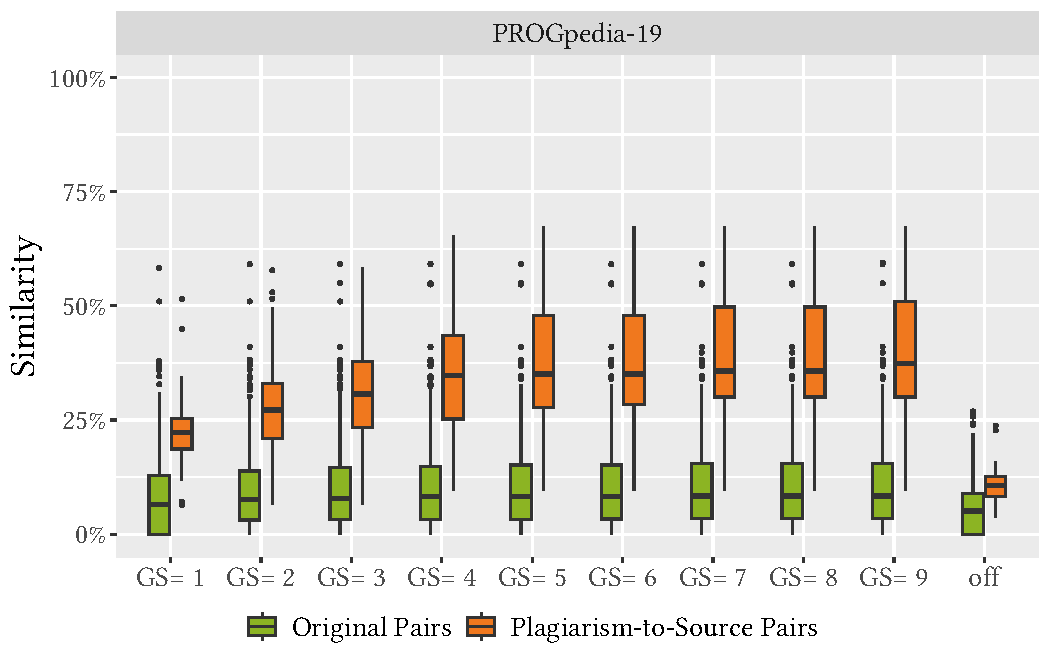
\includegraphics[width=0.95\linewidth]{figures/algorithm/eval-mm-GS_avg.similarity.pdf}
\caption[Impact of the Gap Size]{Impact of the hyperparameter gap size (GS) for a programming assignment dataset~\cite{paiva2023} and plagiarized programs via insertion-based obfuscation via PlagGen~\cite{Broedel2023}. Plagiarism pairs should be high, while original pairs should be low.}
\label{fig:mm-gs}
\end{figure}


\subsection{Limitations}\label{sec:smm-limits}

While subsequence match merging is an effective defense mechanism against various obfuscation attacks, there are some limitations to consider. In the following, we discuss the heuristic nature of the defense mechanism and the choice of suitable hyperparameter values.

    \subsubsection{Heuristic-based Defense}
    The strength of subsequence match merging is that it employs a heuristic to determine which matches to merge.
    Thus, it can provide broad obfuscation resilience, as it requires no knowledge of the specifics of obfuscation attacks.
    However, employing heuristics carries an inherent risk of increasing similarity for unrelated programs, as merging unrelated matches can inadvertently connect unrelated code fragments. This can be the case when a pair of unrelated programs has two sections that are coincidentally similar, and which are separated by a few lines of code in one or both of the programs that are not similar.
    To minimize the impact of match merging on pairs of unrelated programs, we use the original matches whenever too few merging operations are conducted. This significantly reduces the effect on unrelated programs, as for obfuscated programs, many merging operations occur (for example, three to four merges for unrelated programs versus 74 for obfuscated ones, as discussed in \autoref{sec:smm-impact}). 
    Although this mechanism minimizes false positives, subsequence match merging may still slightly increase the similarity of unrelated program pairs.

    \subsubsection{Choice of Hyperparameters}
    We intentionally avoided designing a defense mechanism that relies on too many hyperparameters, as it is always challenging for users to determine an optimal configuration in such cases~\cite{Schmid2022}.
    However, subsequence match merging relies on two hyperparameters (minimum neighbor length and maximum gap size) to determine which subsequences to merge. With a lower minimum neighbor length and a larger maximum gap size, the defense mechanism can revert the effects of stronger obfuscation attacks. However, it is also more prone to merging subsequences that do not belong together, meaning their corresponding code fragments are separated by correctly unmatched code (see \autoref{sec:smm-impact}).
    Incorrect parameter tuning could lead to missed plagiarism cases (under-merging) or excessive false positives (over-merging). To address this issue, we conducted a systematic hyperparameter search on different datasets. We observed that for our datasets, the effects of the hyperparameters are not strong enough to make under-merging or over-merging a probable issue. Specifically, we observed that the hyperparameters mainly affected how well the defense mechanism performed, but the overall detection quality did not fall below the base case, with subsequence match merging disabled.
    From this hyperparameter search, we derived recommended default values for the hyperparameters.
    While these values work well for various datasets, one limitation is that these values are not guaranteed to work for all datasets.
    However, as they are hyperparameters, they can be adapted to the specific dataset at hand.
    